% GNUPLOT: LaTeX picture with Postscript
\begingroup
  \makeatletter
  \providecommand\color[2][]{%
    \GenericError{(gnuplot) \space\space\space\@spaces}{%
      Package color not loaded in conjunction with
      terminal option `colourtext'%
    }{See the gnuplot documentation for explanation.%
    }{Either use 'blacktext' in gnuplot or load the package
      color.sty in LaTeX.}%
    \renewcommand\color[2][]{}%
  }%
  \providecommand\includegraphics[2][]{%
    \GenericError{(gnuplot) \space\space\space\@spaces}{%
      Package graphicx or graphics not loaded%
    }{See the gnuplot documentation for explanation.%
    }{The gnuplot epslatex terminal needs graphicx.sty or graphics.sty.}%
    \renewcommand\includegraphics[2][]{}%
  }%
  \providecommand\rotatebox[2]{#2}%
  \@ifundefined{ifGPcolor}{%
    \newif\ifGPcolor
    \GPcolortrue
  }{}%
  \@ifundefined{ifGPblacktext}{%
    \newif\ifGPblacktext
    \GPblacktextfalse
  }{}%
  % define a \g@addto@macro without @ in the name:
  \let\gplgaddtomacro\g@addto@macro
  % define empty templates for all commands taking text:
  \gdef\gplbacktext{}%
  \gdef\gplfronttext{}%
  \makeatother
  \ifGPblacktext
    % no textcolor at all
    \def\colorrgb#1{}%
    \def\colorgray#1{}%
  \else
    % gray or color?
    \ifGPcolor
      \def\colorrgb#1{\color[rgb]{#1}}%
      \def\colorgray#1{\color[gray]{#1}}%
      \expandafter\def\csname LTw\endcsname{\color{white}}%
      \expandafter\def\csname LTb\endcsname{\color{black}}%
      \expandafter\def\csname LTa\endcsname{\color{black}}%
      \expandafter\def\csname LT0\endcsname{\color[rgb]{1,0,0}}%
      \expandafter\def\csname LT1\endcsname{\color[rgb]{0,1,0}}%
      \expandafter\def\csname LT2\endcsname{\color[rgb]{0,0,1}}%
      \expandafter\def\csname LT3\endcsname{\color[rgb]{1,0,1}}%
      \expandafter\def\csname LT4\endcsname{\color[rgb]{0,1,1}}%
      \expandafter\def\csname LT5\endcsname{\color[rgb]{1,1,0}}%
      \expandafter\def\csname LT6\endcsname{\color[rgb]{0,0,0}}%
      \expandafter\def\csname LT7\endcsname{\color[rgb]{1,0.3,0}}%
      \expandafter\def\csname LT8\endcsname{\color[rgb]{0.5,0.5,0.5}}%
    \else
      % gray
      \def\colorrgb#1{\color{black}}%
      \def\colorgray#1{\color[gray]{#1}}%
      \expandafter\def\csname LTw\endcsname{\color{white}}%
      \expandafter\def\csname LTb\endcsname{\color{black}}%
      \expandafter\def\csname LTa\endcsname{\color{black}}%
      \expandafter\def\csname LT0\endcsname{\color{black}}%
      \expandafter\def\csname LT1\endcsname{\color{black}}%
      \expandafter\def\csname LT2\endcsname{\color{black}}%
      \expandafter\def\csname LT3\endcsname{\color{black}}%
      \expandafter\def\csname LT4\endcsname{\color{black}}%
      \expandafter\def\csname LT5\endcsname{\color{black}}%
      \expandafter\def\csname LT6\endcsname{\color{black}}%
      \expandafter\def\csname LT7\endcsname{\color{black}}%
      \expandafter\def\csname LT8\endcsname{\color{black}}%
    \fi
  \fi
  \setlength{\unitlength}{0.0500bp}%
  \begin{picture}(7200.00,4320.00)%
    \gplgaddtomacro\gplbacktext{%
      \csname LTb\endcsname%
      \put(946,704){\makebox(0,0)[r]{\strut{} 0}}%
      \put(946,1076){\makebox(0,0)[r]{\strut{} 50}}%
      \put(946,1449){\makebox(0,0)[r]{\strut{} 100}}%
      \put(946,1821){\makebox(0,0)[r]{\strut{} 150}}%
      \put(946,2193){\makebox(0,0)[r]{\strut{} 200}}%
      \put(946,2566){\makebox(0,0)[r]{\strut{} 250}}%
      \put(946,2938){\makebox(0,0)[r]{\strut{} 300}}%
      \put(946,3310){\makebox(0,0)[r]{\strut{} 350}}%
      \put(946,3683){\makebox(0,0)[r]{\strut{} 400}}%
      \put(946,4055){\makebox(0,0)[r]{\strut{} 450}}%
      \put(1078,484){\makebox(0,0){\strut{} 0}}%
      \put(2047,484){\makebox(0,0){\strut{} 0.02}}%
      \put(3016,484){\makebox(0,0){\strut{} 0.04}}%
      \put(3985,484){\makebox(0,0){\strut{} 0.06}}%
      \put(4954,484){\makebox(0,0){\strut{} 0.08}}%
      \put(5923,484){\makebox(0,0){\strut{} 0.10}}%
      \put(6055,704){\makebox(0,0)[l]{\strut{}$-2\pi$}}%
      \put(6055,1542){\makebox(0,0)[l]{\strut{}$-\pi$}}%
      \put(6055,2380){\makebox(0,0)[l]{\strut{} 0}}%
      \put(6055,3217){\makebox(0,0)[l]{\strut{}$\pi$}}%
      \put(6055,4055){\makebox(0,0)[l]{\strut{}$2\pi$}}%
      \put(176,2379){\rotatebox{-270}{\makebox(0,0){\strut{}Amplitude von $j$ [Fr/s/cm$^2$]}}}%
      \put(6692,2379){\rotatebox{-270}{\makebox(0,0){\strut{}Phase von $j$ [rad]}}}%
      \put(3500,154){\makebox(0,0){\strut{}Radius $\rho$ [cm]}}%
      \put(3500,3945){\makebox(0,0){\strut{}}}%
    }%
    \gplgaddtomacro\gplfronttext{%
      \csname LTb\endcsname%
      \put(4936,1097){\makebox(0,0)[r]{\strut{}\footnotesize Amplitude}}%
      \csname LTb\endcsname%
      \put(4936,877){\makebox(0,0)[r]{\strut{}\footnotesize Phase}}%
    }%
    \gplbacktext
    \put(0,0){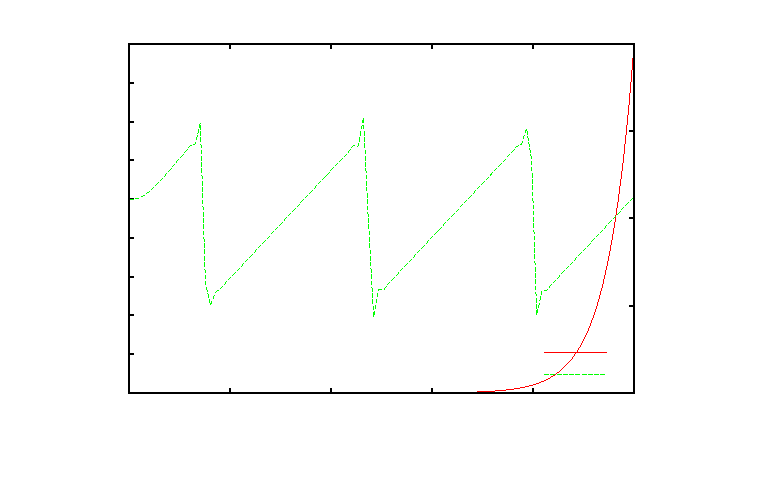
\includegraphics{./figures/e7}}%
    \gplfronttext
  \end{picture}%
\endgroup
